%
% thEvaluator
% Abschlussarbeit (Bachelor)
%
% Thema: Erstellung einer Browser Extension zur Usability Evaluierung von beliebigen Web-Applikationen über Heatmaps.
% Betreuer 1: Prof. Dr. Targo Pavlista
% Betreuer 2: Siamak Haschemi
%
% @author Christian Bromann <contact@christian-bromann.com>
%

\chapter{thEvaluator}

Schon lange entwickelt sich das Web Tag für Tag weiter. Neue APIs werden veröffentlicht und neue Methoden zur Erstellung von noch komplexeren Webapplikationen ausprobiert. Unglücklicherweise schöpfen Usability-Tools diese Technologien nicht immer ausreichend aus und verbauen sich dadurch die Möglichkeit, mehr aus dem Verhalten von Besuchern zu erfahren. Vergleicht man die Tools, die bereits auf dem Markt zu finden sind, so gibt es außer Click- oder Heatmaps kaum andere Features, die einem erklären können, wie die Seite wirklich genutzt wird und wo es Schwachstellen im Interface gibt. Im Rahmen dieser Bachelor Arbeit ist deshalb ein Tool entstanden, welches die positiven Aspekte der bereits veröffentlichten Tools vereint und dabei auf den neuesten Web-Technologien aufsetzt.\\
\\
\textit{thEvaluator}\footnote{Projektwebsite zu finden auf \url{http://qcentral.org}} ist ein aufgabenbasiertes Tool, welches das Usability-Testing mit den neuesten Webstandards vereint. Es ist in der Lage, jede beliebige Website zu testen und verzichtet auf jegliche Anforderungen an den Benutzer des Tools, irgendwelche Code Schnipsel in eine externe Seite einzufügen. Usability-Tests werden dadurch für jeden einfach zugänglich. Durch den aufgabenbasierten Charakter der Software ist kein Usability-Experte zur Analyse der Ergebnisse zwingend erforderlich, um die Intention des Benutzers zu bestimmen. Die aufgezeichneten Daten werden in verschiedenster Form visualisiert, um das Erkennen von Problemen zu vereinfachen.\\
\\
Eine Webapplikation bietet die Oberfläche zum Erstellen und Verwalten von Testcases. Diese werden mit einer einzigartigen ID gekennzeichnet. Nachdem ein Testcase mit diversen Aufgaben erstellt wurde, wird die ID an alle zu testenden User verschickt. Diese benötigen zum Start des Tests eine Browser Extension. Um den Umfang der Arbeit nicht zu sprengen, gibt es diese Extension vorerst nur für den Google Chrome Browser\footnote{\url{http://www.google.com/chrome/}}. Nachdem der User die Erweiterung installiert und den Code in die Extension eingegeben hat, startet der Test. Ein neuer Tab mit der zu testenden Seite wird geöffnet. Der User bekommt anschließend eine Aufgabe nach der anderen gestellt. Dabei wird aufgezeichnet, wie er die Seite nutzt und welche Wege er zum Lösen der Task geht.

%
% Zielbestimmungen
% Abschlussarbeit (Bachelor)
%
% Thema: Erstellung einer Browser Extension zur Usability Evaluierung von beliebigen Web-Applikationen über Heatmaps.
% Betreuer 1: Prof. Dr. Targo Pavlista
% Betreuer 2: Siamak Haschemi
%
% @author Christian Bromann <contact@christian-bromann.com>
%

\newglossaryentry{DOM}{name=DOM, description={Entspricht dem \textit{Document-Object-Model} und bezeichnet das HTML Gerüst einer Webseite}}

\section{Zielbestimmungen}

Das Ziel ein Tool entwickeln, welches die Usability einer Webseite untersuchen soll, setzt nicht gleich dessen Funktionsweise und Handhabung voraus. Es müssen Entscheidungen getroffen werden, die richtungsweisend dafür sind, wie das Tool später benutzt wird. Diese Entscheidungen müssen wohl überlegt sein, da Usability auch sehr entscheidend für eine Software ist, die die Usability analysiert. Die Definition einer Zielgruppe ist dabei ein sehr wichtiger Faktor in der Entscheidungsfindung. \textit{thEvaluator} ist dafür entwickelt worden, um das Usability Testing einfach zu gestalten. Es soll für möglichst viele Personen benutzbar sein und erfordert daher kaum Erfahrungen im Programmieren. Zudem soll die Auswertung ebenfalls einfach gehalten werden, sodass die Benutzer des Tools keinen Usability Experten für die Analyse konsultieren müssen. Die Frage, ob Besucher eine Webseite richtig benutzen und schnell zu ihrem Ziel finden, kann hierbei durch klare Visualisierungen schnell beantwortet werden.\\
\\
Je komplexer eine Programm wird, desto mehr Konfigurationen gibt es, die der User beachten muss. Gute Software zeichnet sich dadurch aus, dass sie zwar viele Konfigurationen anbietet, jedoch nur wenige vom Benutzer wirklich braucht, um zu funktionieren. Um die einfache und schnelle Nutzung des \textit{thEvaluator} Tools zu bewahren, sollte dieses deshalb ohne große Einrichtungsprozesse nutzbar sein. Eine Einschränkung der Funktionalität oder die teilweise Verkomplizierung der Nutzung muss dabei manchmal in Kauf genommen werden. Diese Konzeptionsfragen sind vom Entwickler oder Entwicklerteam jedes mal neu zu evaluieren.\\
\\
Die meisten der bisherigen Usability Tools verlangen vom Nutzer die Einbindung eines Scriptes in die zu testende Seite. Diese Codeschnippsel binden meist eine externe Bibliothek ein, die sich darum kümmert, jegliche Aktionen und Events auf der Seite zu erfassen und an den Server zu schicken. Der Vorteil dieses Verfahrens ist, dass die Testuser einfach nur die Seite besuchen müssen, um am Test teilzunehmen. \textit{thEvaluator} verfolgt hier einen anderen Ansatz. Es erfordert ein Browser Plugin, welches sich um die Datenaufzeichnung kümmert und die Aufgaben des Testcases in die Seite einblendet. Dadurch erfordert es keine Programmierkenntnisse, dieses Tool nutzen zu können. Zudem ermöglicht es das Testen jeder beliebigen Seite im Web. Unzählige Möglichkeiten eröffnen sich dadurch, da nicht nur die eigene Seite analysiert und ausgewertet werden kann, sondern auch die der Konkurrenz. Das Tool ist somit universell einsetzbar. Großer Nachteil an diesem Verfahren ist, dass Testuser dazu aufgefordert werden, sich fremde Software auf ihrem System zu installieren. Dies schreckt im ersten Moment viele ab, was dazu führt, dass weniger Personen an dem Test teilnehmen. Da die Nutzung von Browser-Erweiterungen heut zu Tage jedoch weit verbreitet ist und die Installation von den Herstellern sehr vereinfacht wurde, ist der Nachteil bei Weitem nicht so groß, wie die Möglichkeiten, die durch den universellen Einsatz hervortreten.\\
\\
Eine weitere wichtige Konzeptionsentscheidung ist der Einsatz von aufgabengetriebenden Testcases. Tasks haben einen enormen Einfluss auf Usability Tests. Sie lenken die Besucher auf bestimmte Wege und manipulieren somit gewollt das Userverhalten. Tests können dadurch bestimmte Besucherintentionen simulieren oder sich auf gezielte Bereiche einer Webseite konzentrieren. Nach Hertzum und Jacobson offenbaren verschiedene Typen von Aufgaben unterschiedliche Arten von Usability Problemen. Hingegen strukturierte Aufgaben lediglich Oberfläche Schwachstellen aufdecken \cite{anzahlTestpersonen}. Die Möglichkeiten an Aufgaben sind bei \textit{thEvaluator} daher sehr groß. Ob es ein Klick auf einen Link ist oder das Öffnen des Contextmenüs, jedes vom Browser erzeugte Event kann durch das Tool abgefangen werden. Würde es auf die Aufgaben verzichten und lediglich das Verhalten der alltäglich kommenden Besucher aufzeichnen, so hätte man zwar ein natürlicheres Abbild der Seitennutzung, könnte die einzelnen Intentionen der Besucher jedoch kaum nachvollziehen und dadurch nicht genau erfassen, ob eine Handlung bewusst und gewollt oder unbeabsichtigt war.\\
\\
Der Zeitpunkt wann eine Aufgabe durch den User erfüllt wurde, ist klar zu definieren. Die Browser Extension muss dabei durch die Webseite ein Signal bekommen, wann dies geschehen ist. Diese Signale werden im Web als Events bezeichnet. Die Eventübertragung kann dabei entweder programmatisch durch die Webseite selber erfolgen oder von der Extension übernommen werden. Ersteres hat den Vorteil, dass der Zeitpunkt und die Action des Nutzers besser durch interne Scripte abgefangen werden kann und dadurch individuellere Aufgaben möglich sind. Dies würde aber zusätzlichen Aufwand für die Nutzung des Tools voraussetzen, da dies erst in die Website implementiert werden muss. Zusätzlich wäre man nicht mehr in der Lage, jede beliebige Webseite testen zu lassen, da das Ändern von Code fremder Webseiten nicht möglich ist. \textit{thEvaluator} ist jedoch darauf ausgelegt, möglichst jede Seite testen zu können und dies ohne irgendwelche Änderung am Code. Bei der Erstellung eines Tasks benötigt es deshalb vom User ein Ziel-Event, um eine Aufgabe zu lösen. Dieses Ziel-Event wird durch zwei Komponenten definiert. Zum Einen den Typ des Events und zum Anderen das \Gls{DOM}-Element, welches das Event erzeugen soll. Mit diesen Informationen kann die \textit{thEvaluator}-Extension bei jeden Seitenaufruf einen Listener registrieren, der darauf reagiert, wenn der Browser das definierte Event sendet. Eine mögliches Ziel-Event könnte z.B. der Klick auf ein \Gls{DOM}-Element vom Typ Link sein, welcher als Ziel eine bestimmte Seite attributiert. Diese Art der Zieldefinierung schränkt zwar die Individualität der Aufgaben ein, da z.B. keine Eingabeevaluierungen möglich sind oder auf bestimmte Seitenzustände nicht reagiert werden kann, dennoch ermöglicht es das Realisieren von vielen grundlegenden Aufgaben, wie das Finden von Informationen auf bestimmten Unterseiten. Zudem ist es möglich die Ziel-Events trotzdem in die Seite zu implementieren und dadurch die Aufgaben für den Test zu individualisieren.
%
% Produkteinsatz
% Abschlussarbeit (Bachelor)
%
% Thema: Erstellung einer Browser Extension zur Usability Evaluierung von beliebigen Web-Applikationen über Heatmaps.
% Betreuer 1: Prof. Dr. Targo Pavlista
% Betreuer 2: Siamak Haschemi
%
% @author Christian Bromann <contact@christian-bromann.com>
%

\section{Produkteinsatz}

Für eine erfolgreiche Evaluierung der Usability einer Website mit \textit{thEvaluator} werden als erstes Probanden benötigt, die bereit sind, sich die Extension zu installieren und den Test durchzuführen. Die Anzahl der Teilnehmer sollte zwischen 5 und 15 Personen liegen. Als nächstes muss der Testcase und die darin enthaltenen Aufgaben definiert werden. Die Aufgaben sollten klug gewählt sein und den Proband auf mögliche Usability Problemstellen leiten. Wichtig ist auch, dass die Fragestellung klar und verständlich formuliert wird. Der User sollte beim Test sofort wissen, was er tun muss. Die Reihenfolge der Aufgabe spielt hier eine wichtige Rolle. Der Test sollte, wenn möglich, eine Art Geschichte erzählen, die den User dazu bringt sich besser in die Situation hineinzuversetzen.\\
\\
Die Geschichte kann dabei Situationen beinhalten, dessen Ausgang die Fortsetzung bestimmt. Scheitert der User an einer bestimmten Aufgabe, so kann es vorkommen, dass die Folgeaufgaben nicht ausführbar sind. Es ist deshalb möglich, eine Aufgabe als \glqq erforderlich\grqq{} zu markieren. Dadurch wird der Test beendet, wenn der User es nicht schafft die Aufgabe zu lösen. Dieser wird dann dementsprechend auch in der Auswertung als \glqq durchgefallen\grqq{} gekennzeichnet. Bei einem Usability Test eines Shopsystems kann der User bspw. keine Bestellung durchführen, wenn er es nicht einmal schafft, einen Artikel in den digitalen Warenkorb zu legen.\\
\\
Eine weitere Komponente einer Aufgabe ist die Zeit. Der Benutzer sollte nicht zu lange brauchen einen Task zu erfüllen. In einer realen Situation würde dieser die Seite irgendwann verlassen, da er ungeduldig wird und sein Glück auf einer anderen Webseite sucht. Die Zeit ist deshalb eine Faktor dafür, ob die Aufgabe bestanden ist oder nicht. Läuft sie ab, so endet der Task und der nächste startet automatisch. Ist die Aufgabe jedoch als \glqq erforderlich\grqq{} markiert, so endet der Test.\\
\\
Nachdem die Aufgaben zusammengestellt und der Testcase erzeugt wurde, bekommt diese eine 10-stellige ID zugewiesen. Dies ist der Schlüssel zum Starten des Tests. Er sollte mit ein paar Erläuterungen an die Testuser geschickt werden. Diese geben den Code in die Extension ein und beginnen damit den Test. Es öffnet sich ein neuer Tab mit der im Testcase definierten Seite. Sobald diese geladen ist wird die erste Frage angezeigt. Fortan zeichnet die Extension jegliche Bewegungen der Maus und dessen Klicks auf. Der Test ist beendet, sobald der Benutzer alle Aufgabe erfolgreich gelöst hat oder die Zeit für einen erforderlichen Task abgelaufen ist. Er hat danach noch die Möglichkeit in einem Textfeld individuelles Feedback zu geben und seine Erfahrungen, die er während des Tests gemacht hat, aufzuschreiben.
%
% Komponenten
% Abschlussarbeit (Bachelor)
%
% Thema: Erstellung einer Browser Extension zur Usability Evaluierung von beliebigen Web-Applikationen über Heatmaps.
% Betreuer 1: Prof. Dr. Targo Pavlista
% Betreuer 2: Siamak Haschemi
%
% @author Christian Bromann <contact@christian-bromann.com>
%

\section{Komponenten}

Der Aufbau von \textit{thEvaluator} besteht aus drei Komponenten. Darunter gehören eine Web-Applikation, die es ermöglicht, Testcases zu erstellen und zu verwalten, eine API und Socket-Schnittstelle, die sich um die Persistierung und Ausgabe jeglicher Daten kümmert, sowie einer Browser Extension für den Chrome Browser, die den User durch den Test führt. Abbildung \ref{structure} zeigt, wie diese einzelnen Komponenten miteinander arbeiten. Datenpakete werden dabei entweder via Socket Verbindung oder Ajax Request ausgetauscht.

\begin{center}
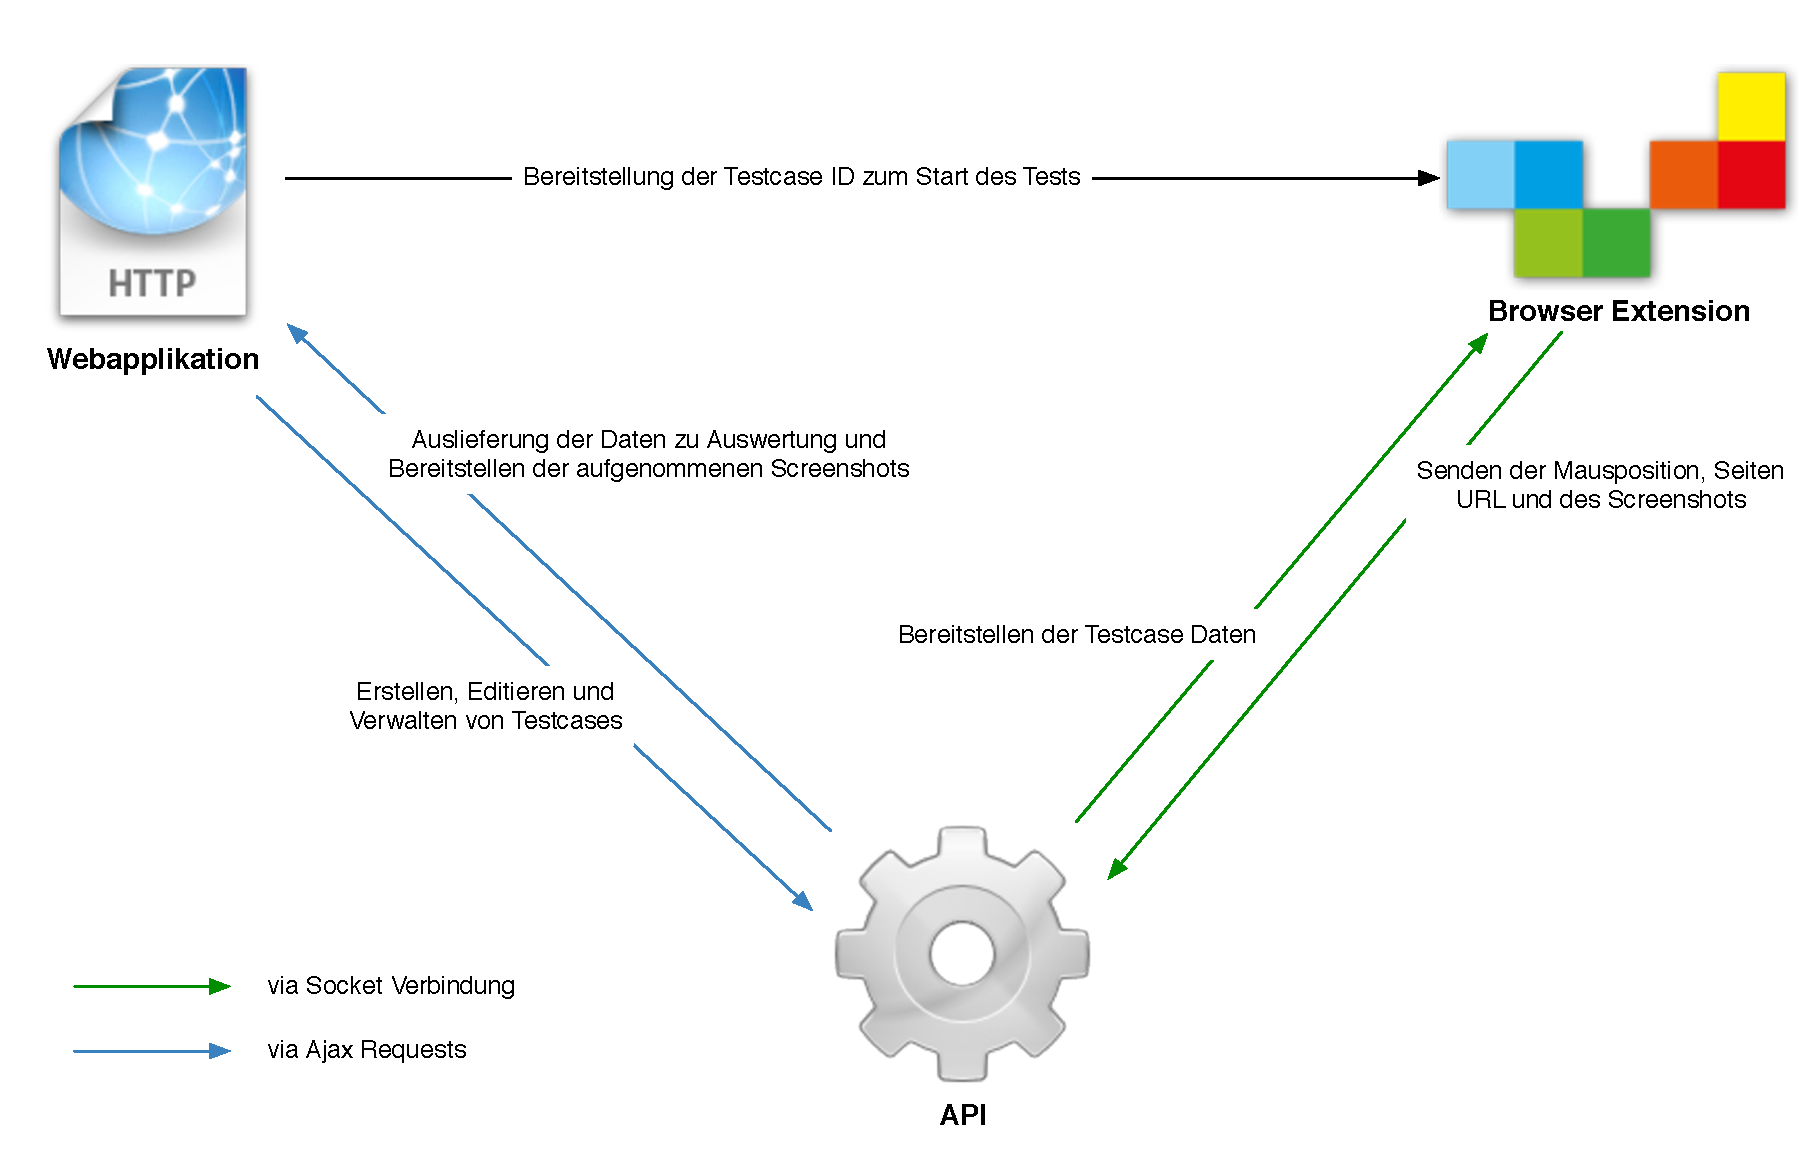
\includegraphics[scale=0.49]{./images/structure}
\end{center}
\begin{figure}[htb]
   \centering
   \caption{Zusammenwirken der einzelnen Komponenten des \textit{thEvaluator} Frameworks}
    \label{structure}
\end{figure}
\newpage
%
% API
% Abschlussarbeit (Bachelor)
%
% Thema: Erstellung einer Browser Extension zur Usability Evaluierung von beliebigen Web-Applikationen über Heatmaps.
% Betreuer 1: Prof. Dr. Targo Pavlista
% Betreuer 2: Siamak Haschemi
%
% @author Christian Bromann <contact@christian-bromann.com>
%

\section{API}

Die \textbf{API} ist der Datenmotor des Frameworks. Sie ist sowohl für die Datenpersistierung als auch für dessen Auslieferung zuständig. Hinter ihr steckt eine NodeJS Applikation, die als dedizierter Service auf einem Server unter einem bestimmten Port laufen muss. Bei einem Test ist sie in ständiger Verbindung mit der Browser Extension, um möglichst viele Daten aufzunehmen. NodeJS eignet sich hierfür sehr gut, da es event-getrieben agiert und dabei nicht blockierend wirkt. Dies bedeutet, dass alle langandauerenden Aktivitäten, wie z.B. Dateizugriffe, Netzwerk Kommunikationen oder Datenbankzugriffe, bei Seite gepackt werden, bis sie beendet sind und das Ergebnis in einer Funktion verarbeitet werden kann \cite{nonblocking}. Dadurch werden Server-Anfragen parallel abgearbeitet und nicht, wie z.B. bei PHP, sequenziell. Dies sorgt für eine stabile Verbindung zwischen Server API und Extension. Zusätzlicher Vorteil einer NodeJS basierten API Architektur ist die Performance. NodeJS basiert auf Googles hochgeschwindigkeits V8 Engine und sorgt damit für eine deutliche höhere Reaktionszeit beim Server im Vergleich zu Apache-Servern \cite{nodevsphp}.


\subsection{Architektur}

% express, welche Models gibt es
% Welche Dependencies , Deploymentprozess

\subsection{Asynchronität in nodeJS}
% Möšglichkeiten zur Lšösung Ÿüber closures, callbacks, Modulen wie async

\subsection{REST Schnittstellen}
% Auflistung mit erforderten Werten / RŸückgabewerten

\subsection{Socket Streams}
% Auflistung mit erforderten Werten / RüŸckgabewerten

\subsection{Persistierung}
% SQL vs NoSQL
% MongoDB / Mongoose
%
% Extension
% Abschlussarbeit (Bachelor)
%
% Thema: Erstellung einer Browser Extension zur Usability Evaluierung von beliebigen Web-Applikationen über Heatmaps.
% Betreuer 1: Prof. Dr. Targo Pavlista
% Betreuer 2: Siamak Haschemi
%
% @author Christian Bromann <contact@christian-bromann.com>
%

\newglossaryentry{MHTML}{name=MHTML, description={MIME Encapsulation of Aggregate HTML Documents - ist die Zusammensetzung einer HTML Seite mit all ihren Ressourcen (referenzierte Skripte werden eingefügt und Bilder als base64 String umgewandelt)}}

\section{Extension}

Für die Durchführung der Tests und der Aufzeichnung der Daten ist die Chrome Extension verantwortlich. Sie muss bei jedem Probanden installiert sein, um am Test teilzunehmen. Dies ist sicherlich zu erst einmal hinderlich, da zum Einen nicht zu erwarten ist, dass ein Testuser diese Extension nutzen möchte, und zum Anderen, dass dieser auch einen Chrome Browser bei sich auf dem System installiert hat. Dennoch ermöglicht es den Nutzern von \textit{thEvaluator}, Testcases für jede beliebige Webseite zu erstellen und aus den Nutzerverhalten dieser zu lernen. Es ist ein Alleinstellungsmerkmal, welches am Ende Vorteile gegenüber Konkurrenzprodukten bringen kann.\\
\\
Da sich die Extension zum Zeitpunkt der Abgabe dieser Arbeit immer noch in einer Art Beta-Phase befindet, wird auf die Einbindung in den Google Web Store\footnote{\url{https://chrome.google.com/webstore}} verzichtet. Für den Beta-Test konnten sich die Probanden die Extension auf der offiziellen Projektwebsite\footnote{\url{http://qcentral.org/}} herunterladen. Da Google es verbietet fremde Extension mit einem einfachen Klick in den Browser einzubinden, muss diese erst heruntergeladen werden und via Drag\&Drop auf die Extensionseite\footnote{\url{chrome://extensions/}} des Browsers gezogen werden. Erst dann wird die Installation von Store-fremden Extensions gestattet. Ist dies erledigt erscheint in der Extension-Bar des Chrome Browsers ein kleines buntes Icon der \textit{thEvaluator}-Erweiterung. Klickt man darauf, so öffnet sich diese in einem kleinen Fenster. Zu sehen ist eine kleine Erläuterung zum Vorgehen des Tests und eine Textbox, in der die Testcase-ID eingegeben werden muss.

\begin{center}
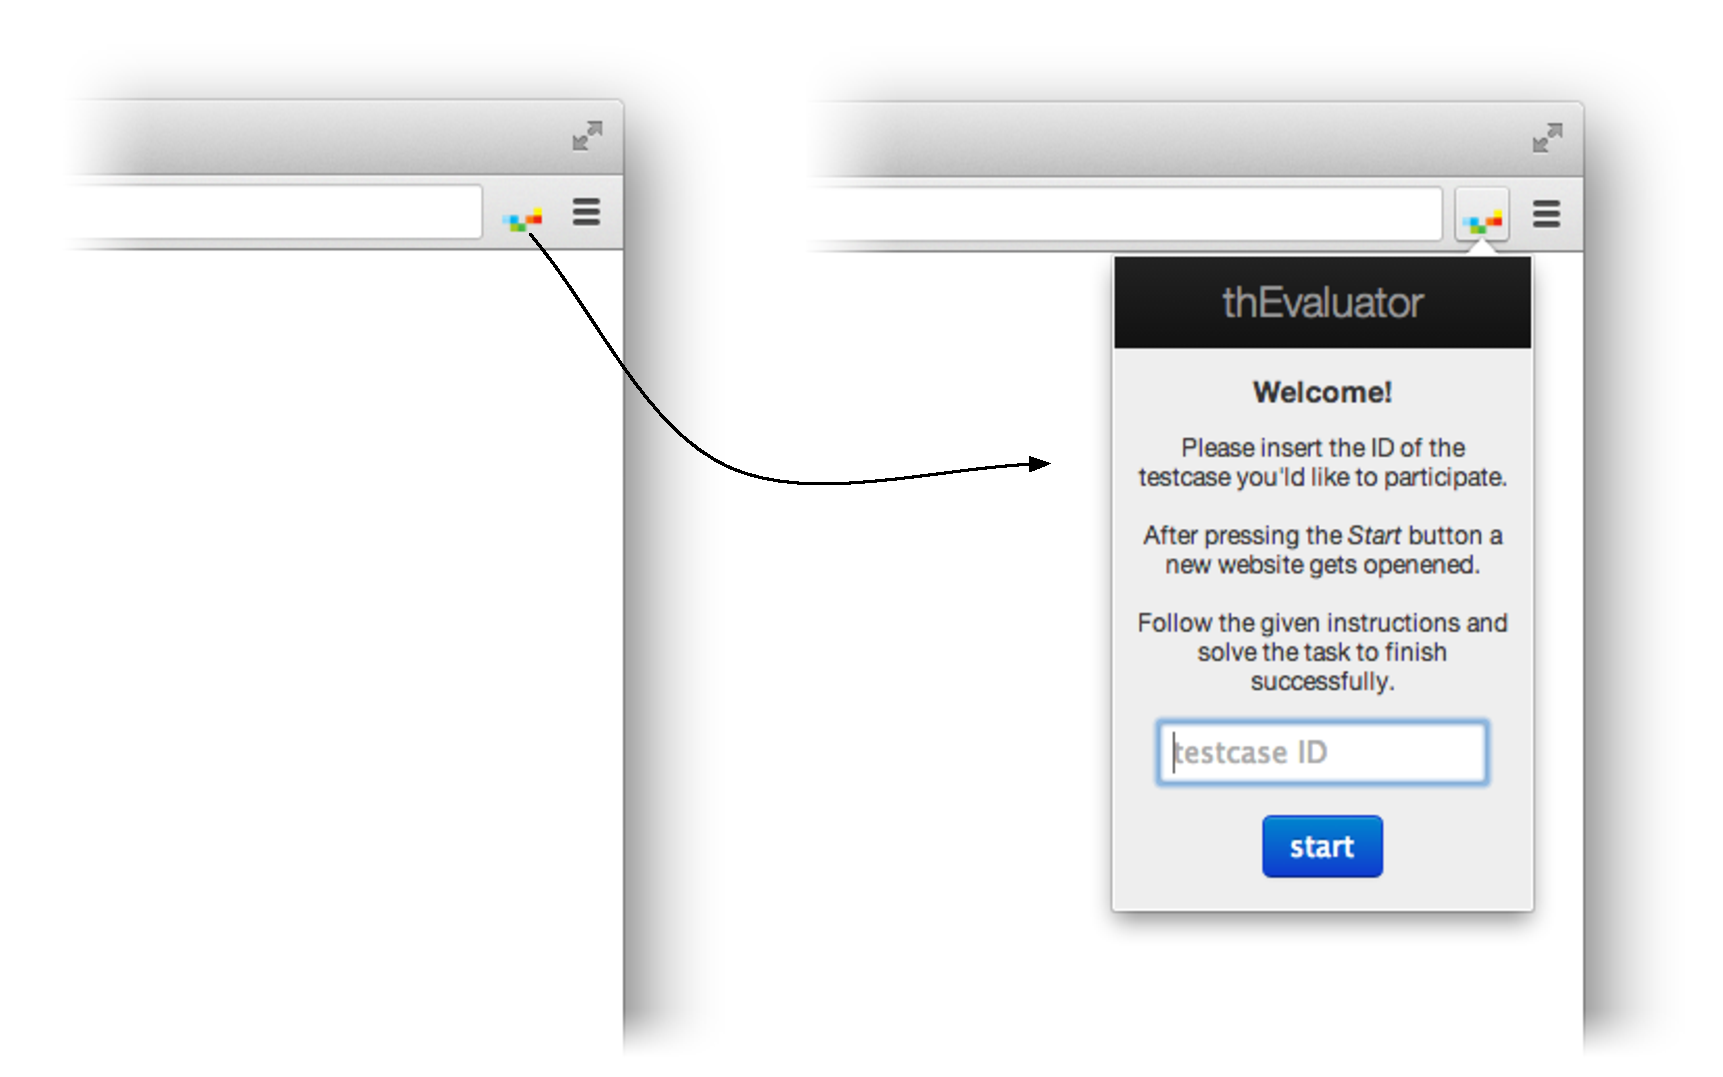
\includegraphics[scale=0.55]{./images/extension}
\end{center}
\begin{figure}[htb]
   \centering
   \caption{Aussehen der \textit{thEvaluator} Extension im Chrome Browser\\nach der Installation}
    \label{extension}
\end{figure}

Sobald der Proband die 10-stellige ID eingegeben hat und den \textit{start} Button drückt, beginnt der Testlauf. Die Extension öffnet dann einen neuen Tab und leitet den User auf die Start-URL.

\subsection{Das Manifest}

Die Inhaltsstoffe einer Chrome Extension sind ganz normale HTML, CSS und JavaScript Dateien. Zusammengehalten wird alles durch ein Manifest, welches die Inhaltsstoffe auflistet und Rechte und Restriktionen festlegt. Jeder Nutzer bekommt bei der Installation angezeigt, welche diese sind und kann entscheiden, ob er sie zulassen möchte. Erst durch die Festlegung ist die Extension in der Lage auf bestimmte Bereiche der API, wie z.B. das Tab-Handling oder die Cookie-Verwaltung, zuzugreifen. Listing \ref{manifest} zeigt einen Auszug des Manifestes der \textit{thEvaluator} Chrome Extension. Neben Name, Versionsnummer und Beschreibung dieser werden Icons definiert sowie HTML Seiten und JavaScripte den jeweiligen Komponenten zugeordnet. Neben diesen Basis-Attributen sind unzählige weitere Angaben möglich, die den Charakter der Erweiterung beschreiben und sie dadurch an verschiedenen Stellen des Chrome Browsers einbetten. Das Manifest muss als JSON Datei im Root-Verzeichnis der Extension liegen.
\\
\begin{lstlisting}[caption=Auszug aus der Manifest.json der \textit{thEvaluator} Extension,label=manifest]
{
    "manifest_version": 2,
    "name": "thEvaluator",
    "version": "0.1",
    "description": "Chrome extension to start thEvaluator usability tests",
    "browser_action":   {
        "default_icon": "img/icon128.png",
        "default_popup": "index.html"
    },
    "icons": { 
        "16": "img/icon16.png",
        "...": "..."
    },
    "background": {
        "page": "background.html"
    },
    "permissions": [ "cookies", "tabs", "http://*/*", "https://*/*" ],
    "content_scripts": [{
        "js": [
            "js/thEvaluatorWidget.js",
            "..."
        ],
        "css": ["dist/injected.css"],
        "all_frames": true
    }],
    "web_accessible_resources": [
        "templates/task.tpl",
        "..."
    ]
}
\end{lstlisting}

\subsection{Generierung durch Grunt}

Eine weitere Komponente der Extension sind die Grunt\footnote{\url{http://gruntjs.com/}} Tasks. Diese kümmern sich um das Testen und Kompilieren der Extension zu einem Paket und die anschließende Umwandlung zu einer Chrome Extension Datei (mit der Endung \textit{.crx}). Grunt ist ein Task-Manager, basierend auf NodeJS, welcher durch Plugins erweitert werden kann und die Entwicklung von Web-Applikationen jeglicher Art automatisiert. Die Tasks werden dabei in einer zentralen Datei, dem Gruntfile, definiert und können jeder Zeit über die Konsole ausgeführt werden. Durch die Kompilierung der Extension durch Grunt werden die CSS und JavaScript Dateien zusammengefügt und minifiziert. Dadurch schrumpft die Dateigröße der Erweiterung und macht den Sourcecode unlesbar. Grundsätzlich ist die Erzeugung der Extension-Datei jedoch auch über den Chrome Browser möglich.

\subsection{Komponenten}

Eine Chrome Erweiterung besteht meist aus drei Komponenten. Einer \textbf{{\color{red}Background Page}}, die im Hintergrund des Browsers ausgeführt wird und die Hauptlogik enthält, einer Seite für die \textbf{{\color{green}Extension UI}}, die für die Ansicht und Logik des Extension-Fensters (PopUp) zuständig ist, und zu guter letzt einem \textbf{{\color{blue}Contentscript}}, die mit der angezeigten Seite des Browser interagieren kann \cite{extensionArchitecture}.

\begin{center}
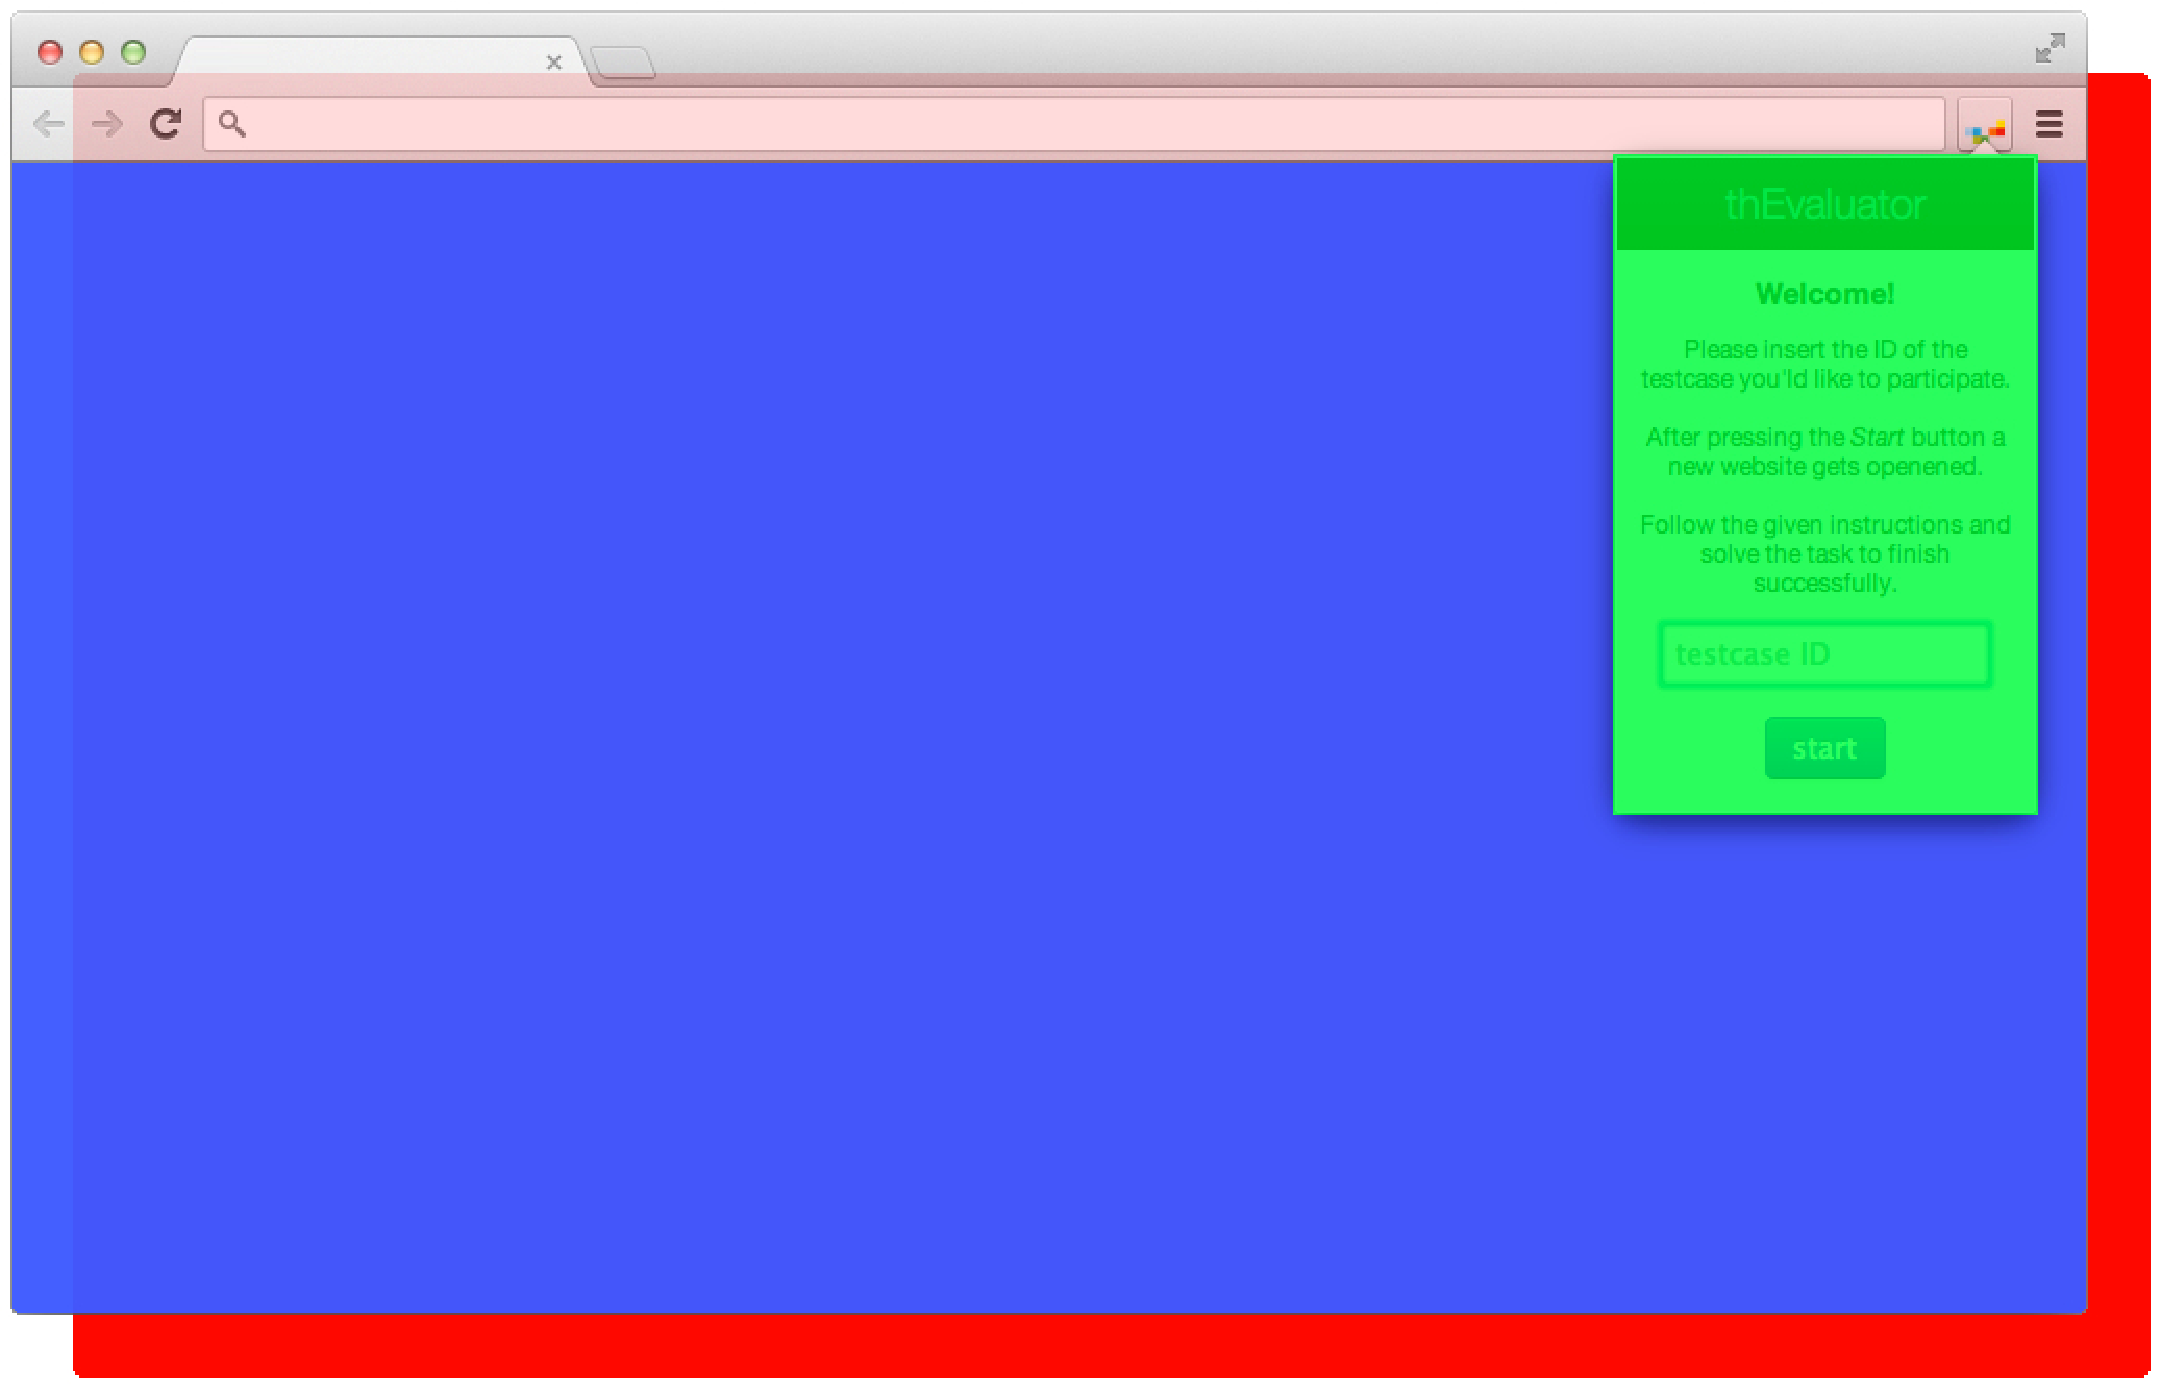
\includegraphics[scale=0.34]{./images/layers}
\end{center}
\begin{figure}[htb]
    \centering
    \caption{Die 3 Komponenten einer Chrome Extension}
    \label{layers}
\end{figure}

Die Laufzeiten der jeweiligen Komponenten sind sehr unterschiedlich. Während die Background Page und dessen JavaScripte dauerhaft ausgeführt werden, passiert dies für den UI Teil erst wenn das PopUp, durch den Klick auf das Extension Icon, geöffnet wird und auch nur die Zeit, solange es geöffnet ist. Das Contentscript dagegen wird immer dann vom Browser ausgeführt, sobald eine neue Seite geladen wird. Es verhält sich somit wie ein Script, welches in jeder Seite eingebunden ist. Es hat es Zugriff auf den DOM der Seite, somit auch auf dessen Struktur, und den Umgebungs- und globalen Variablen.\\
\\
In der \textit{thEvaluator} Extension findet die meiste Aktivität im Contentscript statt. Da die Erweiterung ständig die Mausposition abfragen muss, benötigt es Zugriff auf die globale \textit{window} Variable der Seite. Zudem werden Templates in den DOM gehangen, um eine neue Aufgabe anzuzeigen oder dem User die Information zu geben, welche er gerade bearbeitet. Die UI Page ist dafür verantwortlich die ID des Testcases aufzunehmen und sie anschließend der Background Page zu senden. Konnte die ID erfolgreich identifiziert und zugeordnet werden, wechselt das User Interface und die Aufgabenstellung wird angezeigt. Zusätzlich bietet ein \textit{Stop} Button die Möglichkeit den Testlauf zu beenden. Sobald die Background Page von dem PopUp die ID des Testcases bekommen hat, startet sie eine Socket Verbindung mit dem Server und erhält die Daten des Testcases, sowie dessen Aufgaben. Es öffnet die Start-URL in einem neuen Tab und sendet dem Contentscript eine Nachricht mit den Daten des Testcases. Dieses beginnt nun mit der ersten Frage. Da es nach jedem Seitenaufruf neu initialisiert wird, speichert es seine Umgebungsvariablen, wie zbs. die aktuelle Aufgabennummer, als Cookie ab.


\subsection{Nachrichtenübermittlung}

Die Komponenten der Chrome Extension müssen häufig miteinander kommunizieren. Die Background Page sendet z.B. bei jedem neuen Seitenaufruf die Daten des aktuellen Testcases und initialisiert damit das Contentscript. Dieses sendet jegliche Mauspositionen an die Background Page, damit sie diese via Socket Stream an den Server weiterleiten kann. Die Kommunikation findet dabei über das Message Passing statt \cite{messagePassing}. Jede Komponente kann auf Nachrichten reagieren oder sie selber senden. Dabei ist es sogar möglich Nachrichten an eine andere Extension zu senden, solange dessen ID bekannt ist. Es gibt dabei zwei Arten der Übertragung. Langzeitverbindungen halten einen dauerhaften Kontakt zwischen zwei Komponenten einer Extension. Typischer Use-Case wäre eine Autoformfill-Extension, die bei jeder Eingabe eines Buchstaben im Formular eine Möglichkeit zur Füllung des Formulars anbietet. Die \textit{thEvaluator} Extension nutzt ausschließlich sogenannte \textit{One-Time Requests}. Dabei handelt sich, um einfache Request mit einer JSON Nachricht. Diese besitzen jeweils ein \textit{action} Attribute, die für eine bestimmte Funktion im Contentscript bestimmt ist. Listing \ref{message} zeigt, wie jede Nachricht an eine Funktion im Contentscript zugewiesen wird. Das Objekt, welches diese Funktionen bereitstellt, nennt sich \textit{thEvaluatorInjected} und beinhaltet die Hauptlogik des Contentscripts. Da im Backgroundscript aus Einfachheitsgründen die Funktionen global deklariert werden, regelt eine \textit{switch} Anweisung alle ankommenden Nachrichten.
\\
\begin{lstlisting}[caption=Message Handeling im Contentscript,label=message]
var thEvaluator = new thEvaluatorInjected();
chrome.extension.onMessage.addListener(function(request,sender,sendResponse){

    if(typeof thEvaluator[request.action] === 'function') {
        thEvaluator[request.action](request,sender,sendResponse);
    } else {
        thEvaluator.log('couldn\'t find action: \'' + request.action + '\'');
    }

});
\end{lstlisting}

\subsection{Screenshotaufzeichnung}

Hinter jedem Klick des Users steckt in den häufigsten Fällen ein visuelles Ziel. Ob Link oder Bild, Internetnutzer erkennen ziemlich schnell, wohin man klicken muss, um auf eine neue Seite zu gelangen. Beim durchforsten der Seite ist häufig zu beobachten, dass User die Maus benutzen, um Texte zu erfassen. Der Mauszeiger wird dabei wie eine Art Finger benutzt, der Wort für Wort das Lesen begleitet. Diese visuellen Hintergründe sind daher bei der Auswertung von Heat- oder Clickmaps unersetzlich und helfen die Gründe für das Verhalten des Benutzers herauszufinden. Es ist daher wichtig, das hinter den X und Y Daten ein Bild steckt, zu dem diese zugeordnet werden können.\\
\\
Das Aufnehmen eines Screenshots ist in Google Chrome schwerer als anfangs vermutet. Die API bietet zwar die Möglichkeit, den aktuell sichtbaren Bereich zu scannen, jedoch nicht die komplette Seite. Eine Ausweichmöglichkeit wäre die Erzeugung von \Gls{MHTML} Dateien. Diese würden eine 1 zu 1 Kopie der ursprünglichen Seite abbilden und könnten bei der Auswertung in iFrames angezeigt werden. Da jedoch jegliche Bilder und Skripte in die Datei einfließen, ist der Speicheraufwand zu groß und für das Abscannen vieler Seiten ungeeignet. Daher muss ein Algorithmus die API erweitern, um einen Screenshot der ganzen Seite zu erhalten.\\
\\
In einer Art rekursiven Funktion tastet sich der Algorithmus über die Seite und nimmt sie dabei Stück für Stück auf. Dies geschieht im Skript der Background Page, da lediglich diese die Rechte zur Nutzung der Funktion besitzt. Ist ein Bereich abgescannt, so erhält das Contentscript die Nachricht ein Stück weiter zu scrollen, um einen neuen Teil der Webseite abzuscannen. Ist die Seite abgescrollt ruft die Funktion einen Callback auf und springt damit aus ihrer Rekursivität. Listing \ref{captureVisibleTab} zeigt als erstes die Funktion, die den sichtbaren Teil des Bildschirms einscannt und das Bild in einem Canvas zwischenspeichert.
\\
\begin{lstlisting}[caption=Funktion zum Abscannen des aktuell sichtbaren Bereiches der Seite,label=captureVisibleTab]
capturePage = function(opt,cb) {

    var x = opt.x,
        y = opt.y;

    console.log('take screenshot on %d , %d',x,y);

    chrome.tabs.getSelected(null, function(tab) {
        chrome.tabs.sendMessage(tab.id, {action: 'scroll', pos: {x:x,y:y}}, function(pos) {
            window.setTimeout(function() {
                chrome.tabs.captureVisibleTab(null, {
                    format: 'jpeg',
                    quality: 10
                }, function(data) {

                    if (data) {
                        var image = new Image();
                        image.src = data;

                        image.onload = function() {
                            screenshot.ctx.drawImage(image, pos.scrollX, pos.scrollY);
                            cb();
                        };
                    }

                });
            },150);
        });
    });

};
\end{lstlisting}

Wie in Zeile 9 zu erkennen ist, wird zuerst eine Nachricht an das Contentscript geschickt, auf eine bestimmte X und Y Position der Seite zu scrollen. Erst danach wird die Funktion zum Aufnehmen des Screenshots in Zeile 11 aufgerufen. Wie Zeile 10 zeigt, geschieht dies durch das \textit{setTimeout} erst nach 150ms. Grund dafür ist die Latenz, die durch das Rendern des neuen Bereiches der Seite entsteht. Da das Scrollen sprunghaft geschieht, braucht der Browser eine kurze Zeit, um die Inhalte anzuzeigen. Beim normalen scrollen fällt dies dem menschlichen Auge nicht auf. Bei einem Test wird der User zwar für eine kurze Zeit irritiert, da er die Scrollbewegung mitbekommt. Da dies jedoch für jede URL nur einmal geschieht, sind davon nur sehr wenige Testuser betroffen. Zudem hat dies keinen direkten Einfluss auf das Nutzerverhalten des Benutzers.\\
\\
Gesteuert wird dies durch die rekursive Funktion, die sich erst beendet, wenn der unterste Bereich der Seite erreicht wurde. Die Rekursivität entsteht dadurch, dass der Callback der Funktion \textit{capturePage} die Funktion selber ist und aufgerufen wird, sobald der Screenshot genommen wurde.
\\
\begin{lstlisting}[caption=Rekursive Funktion die das Abscannen der Seite steuert,label=takeScreenshot]
takeScreenshot = function(opt,cb) {

    var x = opt.x || 0,
        y = opt.y || 0;

    if(y < docDimension.height) {
        capturePage({x:0,y:y}, function() {
            takeScreenshot({x:0, y: y + docDimension.innerHeight }, cb);
        });
    } else {
        cb();
    }
},
\end{lstlisting}
\vspace{0,5cm}

Aktuell wird lediglich die vertikal Achse abgescannt. Da die meisten Webseiten sich in der Vertikalen ausbreiten, reicht dies vorerst aus. Hier könnte jedoch der Algorithmus derart erweitert werden, dass die Funktion erst dann aus der Rekursivität springt, sobald auch die X Achse abgescrollt wurde.
%
% Webapplikation
% Abschlussarbeit (Bachelor)
%
% Thema: Erstellung einer Browser Extension zur Usability Evaluierung von beliebigen Web-Applikationen über Heatmaps.
% Betreuer 1: Prof. Dr. Targo Pavlista
% Betreuer 2: Siamak Haschemi
%
% @author Christian Bromann <contact@christian-bromann.com>
%

\section{Webapplikation}

Die Webapplikation ist die Administrationsoberfläche der gesamten Anwendung. Hier erstellt der User des \textit{thEvaluator} Frameworks die Testcases, passt sie an und wertet sie anschließend aus. Wie es sich für einen administrativen Bereich gehört, sollte dieser passwortgeschützt sein und nur bestimmten Personen Zugang gewähren. Aus zeitlichen Gründen wurde jedoch auf ein User-Management verzichtet. Betritt man die Startseite des Bereiches, so erhält der User eine Übersicht über die bereits angelegten Testcases. Neben dem Namen sind drei Aktionsbuttons zu finden, mit denen man den Testcase bearbeiten, löschen oder dessen Details betrachten kann. Ganz oben neben dem \textit{thEvaluator} Logo befindet sich die Navigation. Diese leitet den Benutzer zum Erstellen oder Evaluieren von Testcases weiter.

\begin{center}
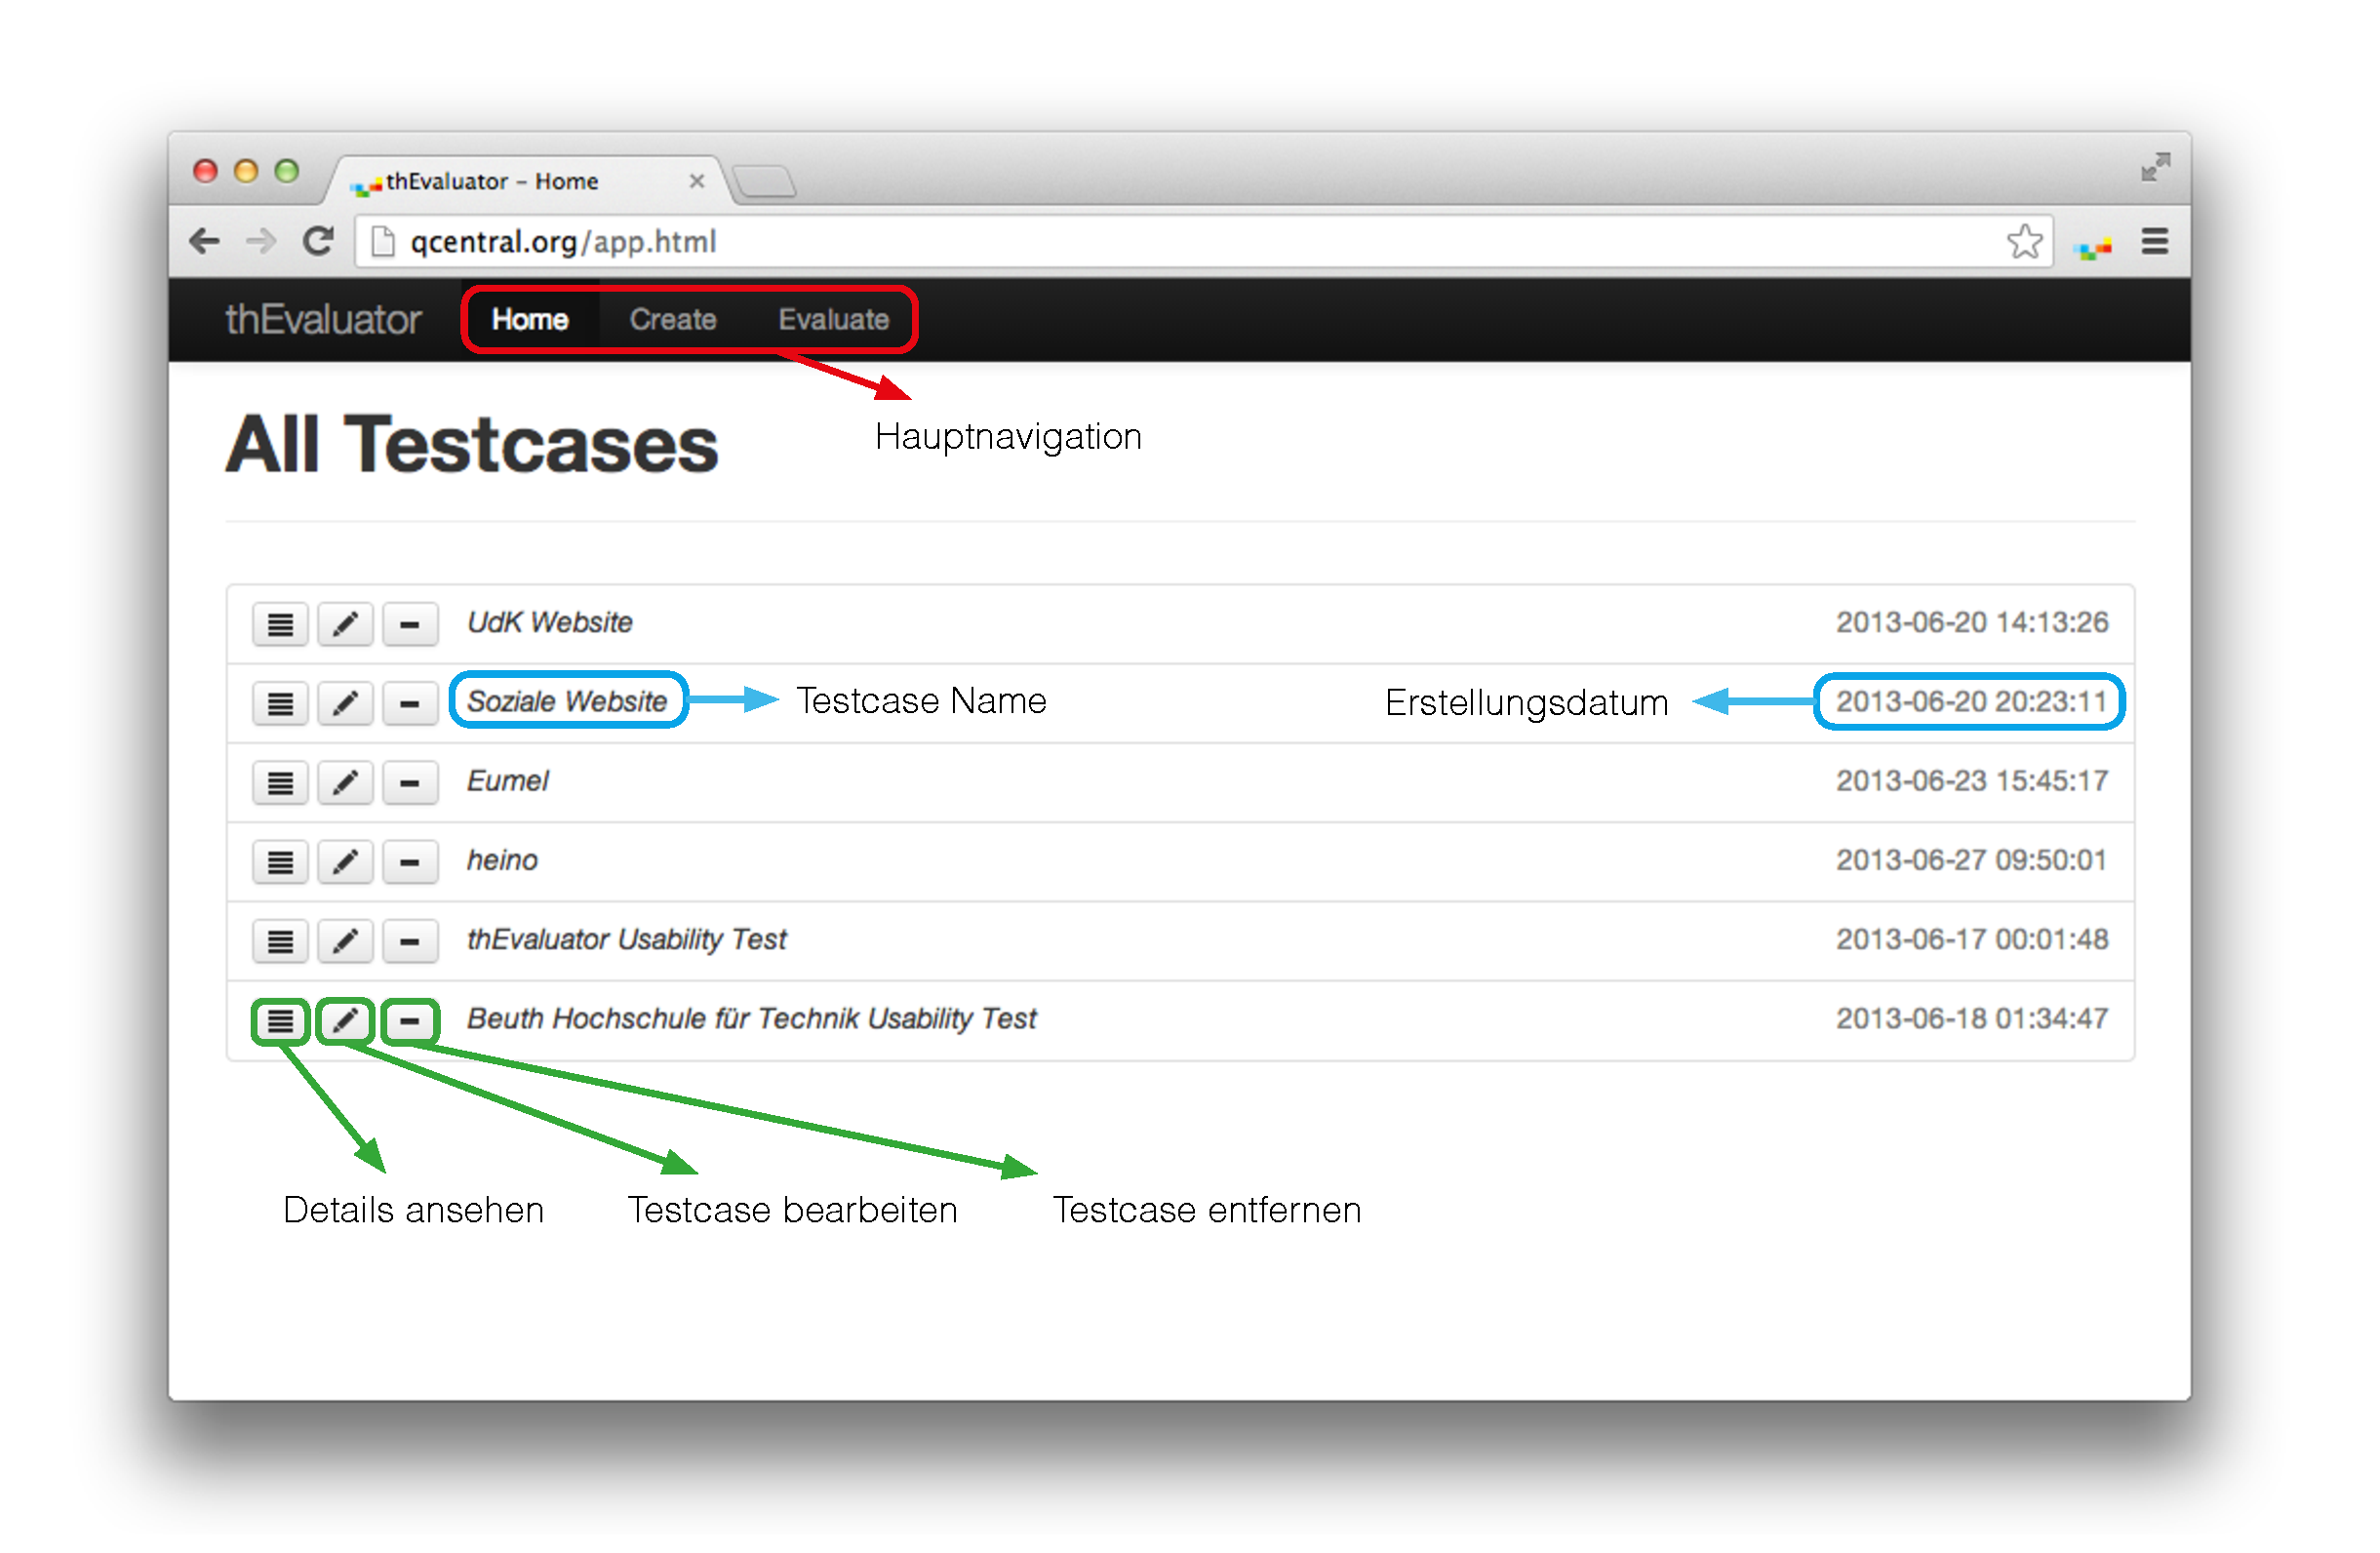
\includegraphics[scale=0.40]{./images/webappscreen}
\end{center}
\begin{figure}[htb]
   \centering
   \caption{Administrationsoberfläche}
    \label{webappview}
\end{figure}

Alles beginnt mit der Erstellung eines Testcases. Es braucht nicht viel Zeit und Eingaben, um einen zu erstellen. Nach dem Klick auf \textit{Create} öffnet sich die Formularansicht. Als erstes vergibt man einen Namen für den Testcase, gefolgt von einer URL. Diese ist der Startpunkt für den Testcase. Es ist dabei nicht notwendig von der Startseite einer Website zu beginnen. Führt man bspw. einen Test für das firmeninterne Intranet durch, so kann auch eine Netzwerk-URL eingegeben werden. Wichtig ist nur, dass die Teilnehmer die notwendigen Rechte zum Zugriff auf die Seite besitzen. Eine weitere wichtige Angabe ist die der Auflösung. Jeder Testcase muss eine feste Auflösung vorschreiben, um die Verhältnisse für jeden Probanden gleich zu setzen. Die Extension verkleinert oder vergrößert beim Starten des Testcases dann automatisch das Browserfenster. Dadurch wird sichergestellt, dass die Testuser unter den gleichen Vorraussetzungen, was Auflösung angeht, die Seite nutzen. Zudem ermöglicht es Usability-Tests für Webseiten mit einem \textit{Responsive Design}. Wählt der User eine Auflösung für mobile Geräte, wie z.B. 320 x 480 px, so erhält er automatisch die Version der Website, die ein mobiler User ebenfalls erhalten würde. Obwohl das Verhalten zwischen Mobil- und Desktop-User dann immer noch nicht das Gleiche ist, bekommt man trotzdem einen recht guten Eindruck davon, wie die mobile Version der Seite genutzt wird.

\begin{center}
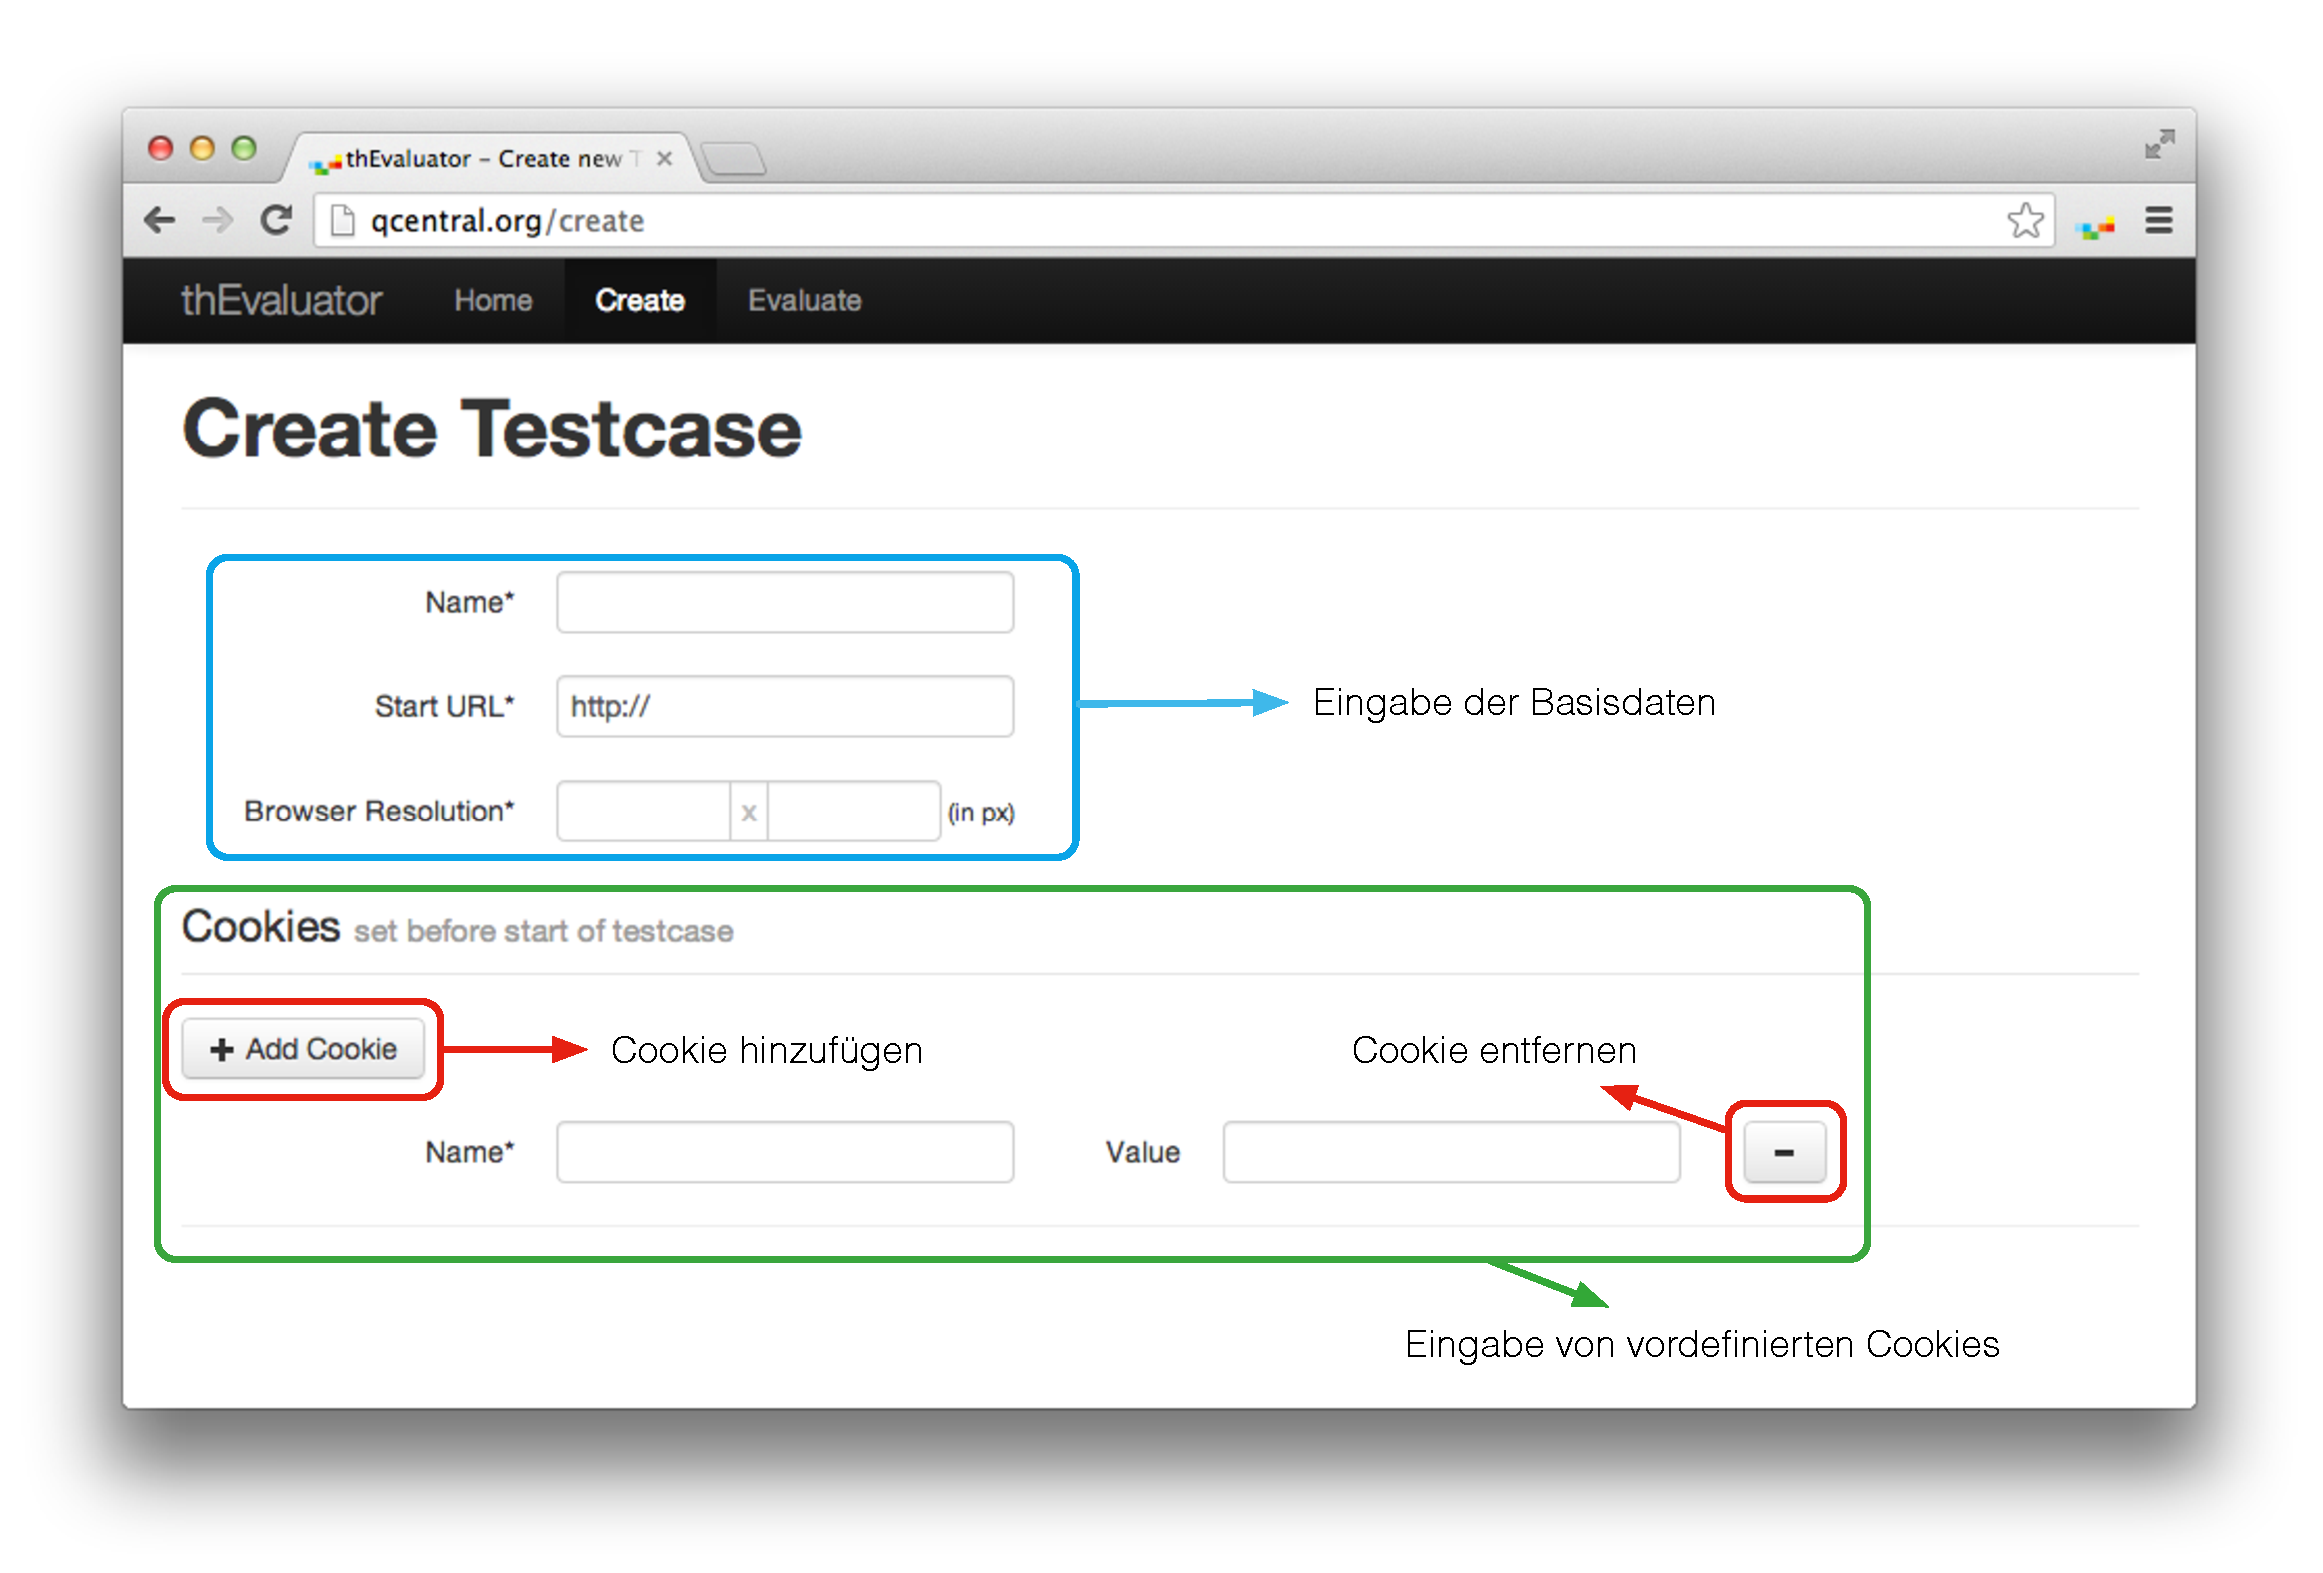
\includegraphics[scale=0.40]{./images/createscreen}
\end{center}
\begin{figure}[htb]
   \centering
   \caption{Formularansicht}
    \label{createview}
\end{figure}

Um den Usability-Test für jeden Bereich einer Webseite möglich zu machen, gibt es zudem die Möglichkeit, Cookies vor dem Start setzen zu lassen. Möchte der User bspw. eine Website testen lassen, die noch nicht veröffentlicht ist, so kann er hier spezielle Cookies definieren, die die Seite erkennt und den Zutritt darauf gewährt. Die Extension setzt diese Cookies vor Beginn des Testcases für alle Subdomains und Pfade der Website. Als letztes werden die Tasks definiert. Diese enthalten, neben dem Namen und einer Aufgabenbeschreibung, ein \textit{required} Feld, welches angibt, ob der Testcase beendet ist, wenn der Proband die Aufgabe nicht lösen kann. Dadurch ist es möglich, eine Aufgabe, wie z.B. die Auswahl eines Produktes im Online-Shop, als Vorraussetzung für die Folgeaufgaben, z.B. die Ware in den Warenkorb zu packen, auszuwählen.

\begin{center}
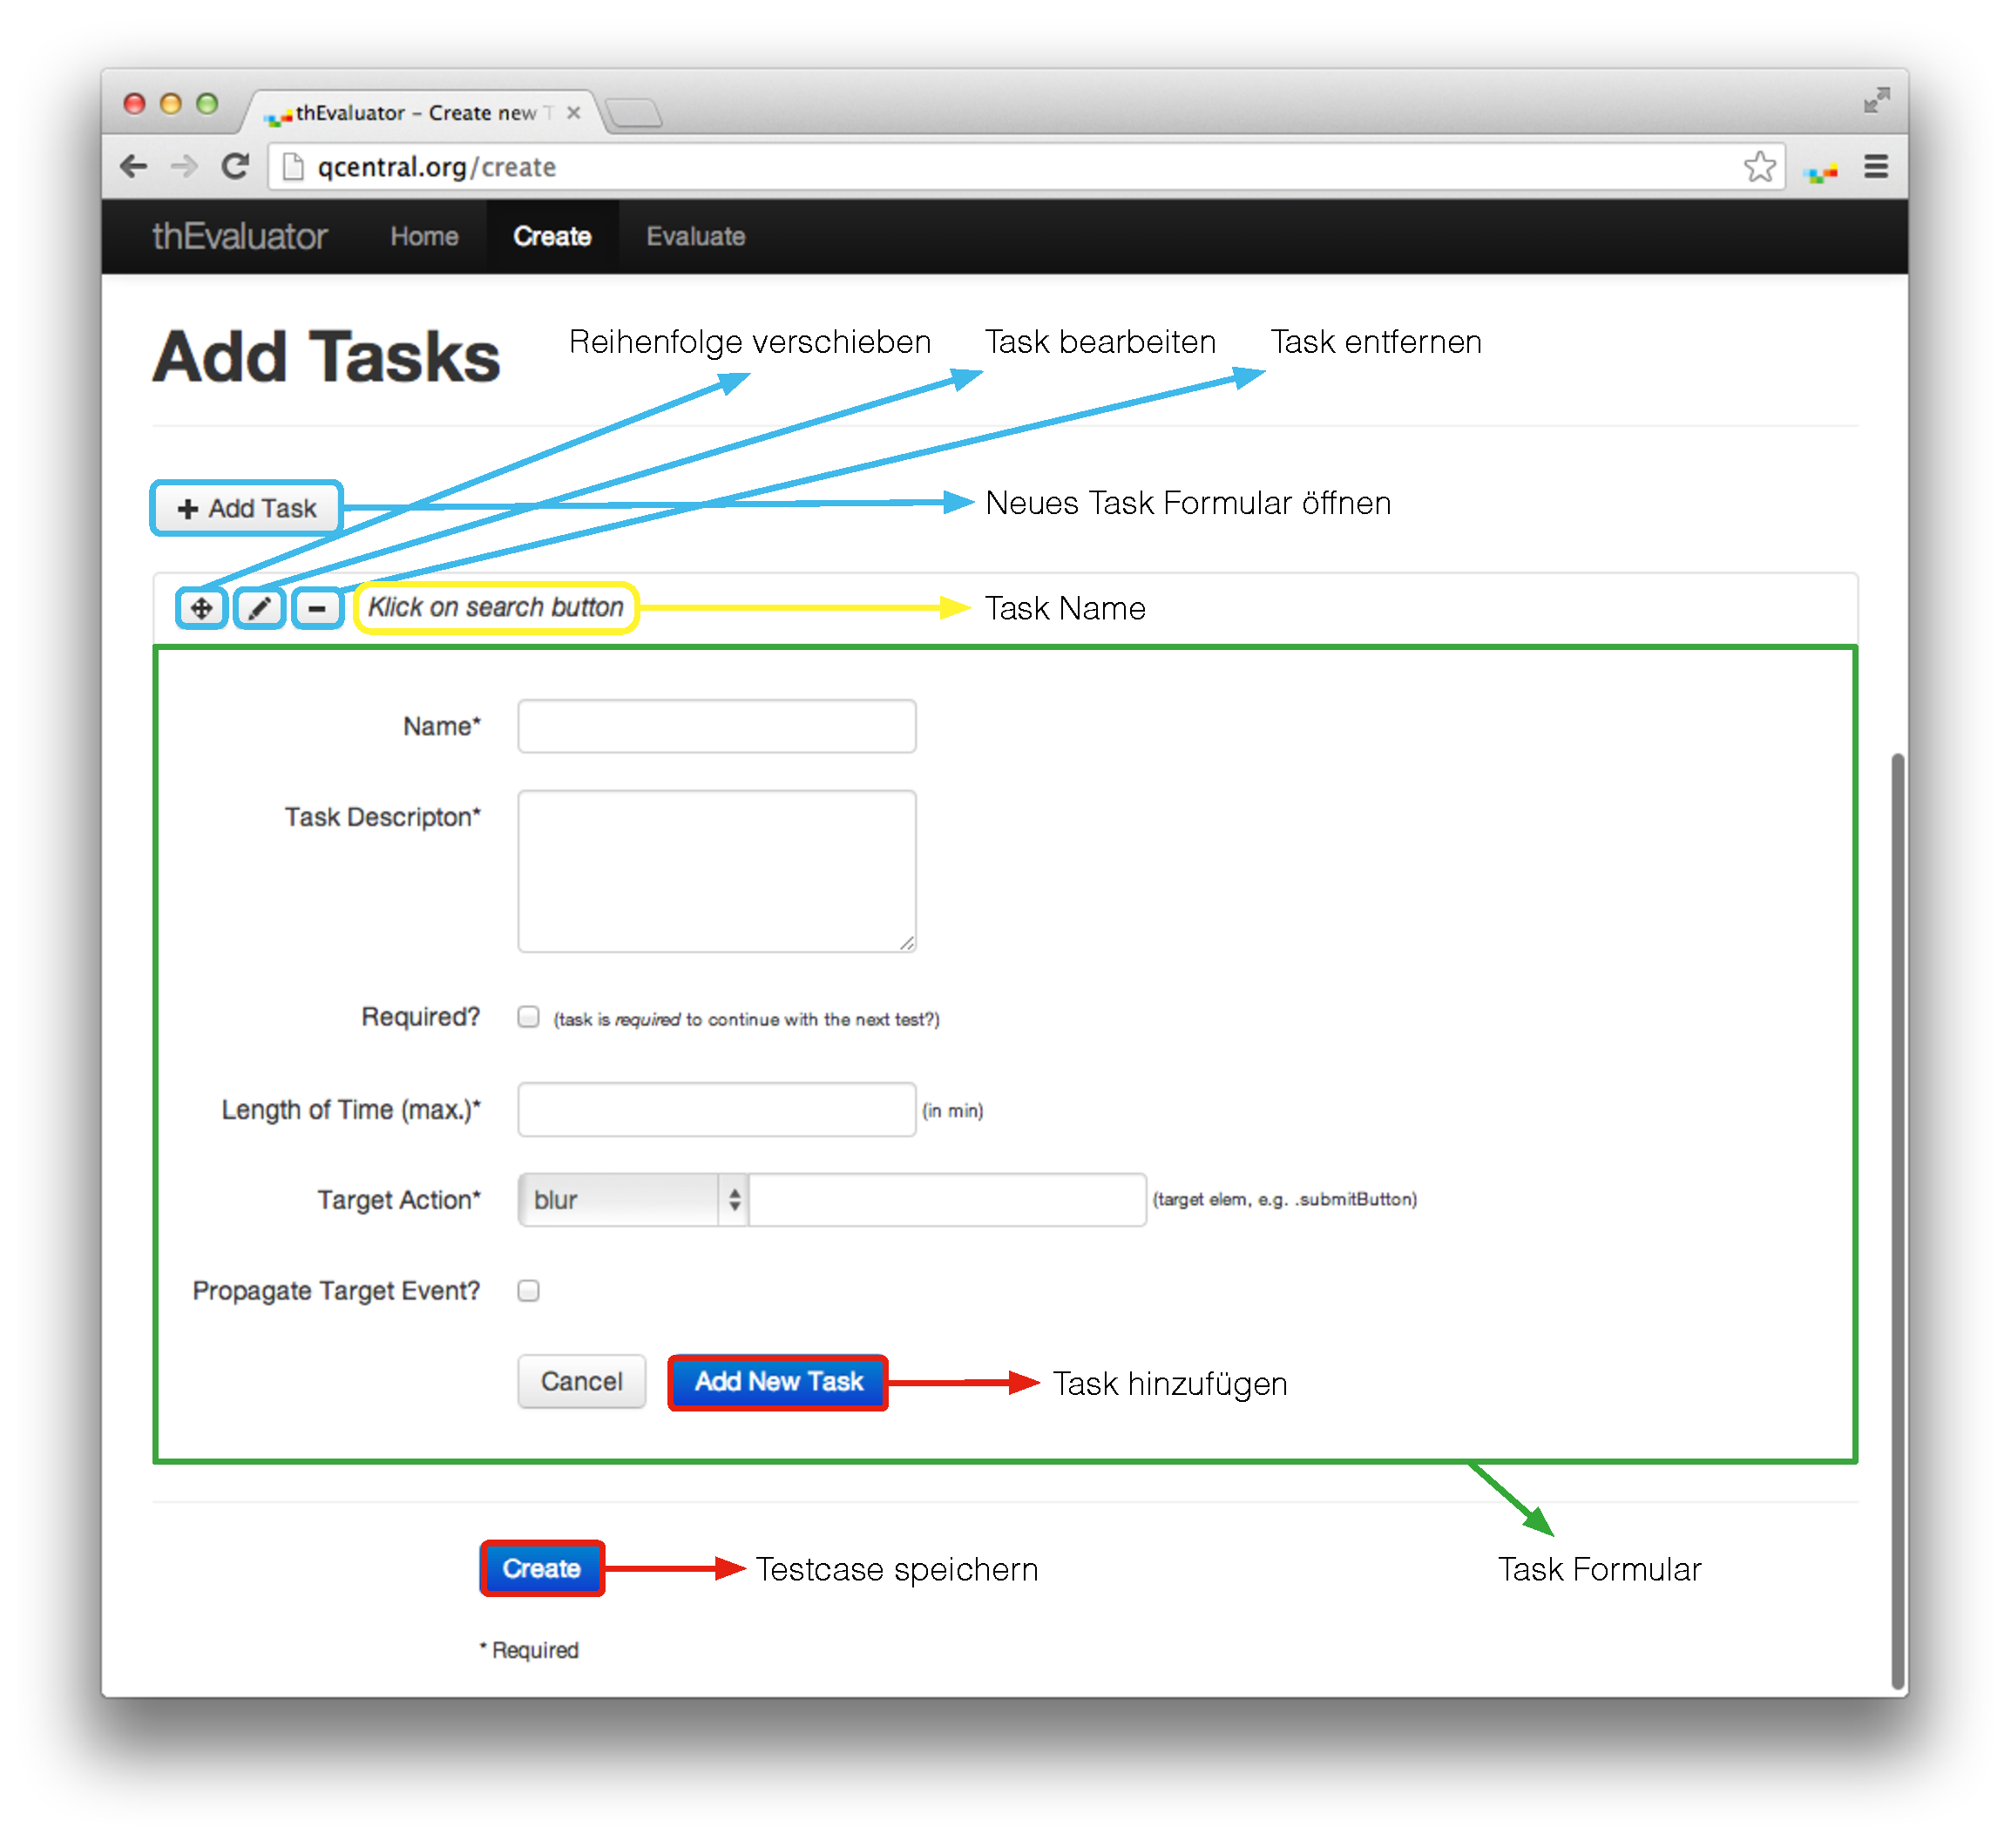
\includegraphics[scale=0.4]{./images/taskscreen}
\end{center}
\begin{figure}[htb]
   \centering
   \caption{Task-Formular}
    \label{taskscreen}
\end{figure}

Ein weiteres Attribut eines Tasks ist die Zeit. Die Aufgabe kann als gescheitert angesehen werden, wenn der Proband zu lange zum Lösen dieser benötigt. In einem realen Szenario würde der User eine Website verlassen, wenn er nach einer bestimmten Zeit nicht an sein Ziel findet. Als nächstes folgt die Angabe des Ziel Events. Dieses besteht, wie in Kapitel \ref{events} beschrieben, besteht dieses aus einer Action und einem Element aus dem DOM. Möchte man bspw. den Klick auf einem Link mit einer bestimmten URL als Ziel einer Aufgabe definieren, so wählt man eine \textit{click}-Action auf einem Element mit dem Selektor \textit{a[href=''\textbf{ URL }'']}. Es kann auf alle CSS3 Selektoren zurückgegriffen werden. Dies macht die Einschränkung der Elemente sehr flexibel. Als letztes ist die Angabe des \textit{Propagation} Attributes möglich. Dies setzt fest, ob das Event, wie z.B. der Klick nach dem Abfangen durch die Extension abgefangen werden soll oder nicht. Bleiben wir beim Beispiel mit dem Klick auf einen Link, so würde sich die neue Seite nur öffnen, wenn die Checkbox aktiviert ist. Der User würde dann mit dem nächsten Task auf dieser Seite weiter machen. Ist die Box nicht aktiviert, so verbleibt er auf der Seite, da die Extension den Klick abfängt, bevor der Browser den Befehl zum Öffnen der neuen Seite bekommt.\\
\\
Nachdem ein paar Aufgaben für den Testcase erstellt wurden, ist im Nachhinein noch möglich, jeden einzelnen Task zu bearbeiten. Zudem kann die Reihenfolge der Aufgaben via Drag\&Drop verschoben werden (siehe \glqq Reihenfolge verschieben\grqq{}-Button in Abbildung \ref{taskscreen}). Als letztes wird der Testcase gespeichert und erhält eine 10-stellige ID, die allen Probanden geschickt werden kann, die an dem Test teilnehmen. Zum Schluss können die Ergebnisse auf der \textit{Evaluate} Seite (siehe Hauptnavigation) ausgewertet. Näheres dazu wird in Kapitel \ref{evaluation} erläutert.


\subsection{Aufbau}

Die Webapplikation des \textit{thEvaluator} Frameworks ist mit den modernsten Frontend-Web-Technologien dieser Zeit entwickelt wurden. Es bedient sich, ebenso wie die Extension-Komponente, dem Grunt Tool für Buildprozesse und Entwicklungsworkflows und nutzt mit Bower\footnote{\url{http://bower.io}} ein Package Manager für das Dependancy-Management. Bereitgestellt wird dieses Set an Tools durch Yeoman\footnote{\url{http://yeoman.io}}. Dieses konfiguriert Grunt und Bower zu einem in sich harmonierenden Workflow und bietet für die Entwicklung verschiedene Scaffolding Möglichkeiten an. Entwickelt wurde dieses System von den erfahrensten Webentwicklern dieser Zeit und einer großen Community, die ständig neue Tools zur Erstellung besserer Webapplikationen entwickelt.\\
\\
Für das Deployment werden verschiedene Dependencies vorausgesetzt. Das System benötigt \textit{Node}, \textit{Ruby} und \textit{Sass\footnote{\url{http://sass-lang.com/}}}. Letztere werden zur Kompilierung der CSS Dateien benötigt. Die Webapplikation nutzt den CSS-Preprozessor Sass, um verschiedene Features, wie z.B. Vererbung oder Verschachtelung der CSS Regeln, nutzen zu können. Das Design baut auf dem bekannten \textit{Twitter-Bootstrap\footnote{\url{http://twitter.github.io/bootstrap/}}} auf und erhält damit ein elegantes Grunddesign, welches flexibel genutzt werden kann. Da die Webapplikation lediglich ein Prototyp ist, wurde auf die Erstellung eines eigenen Designs verzichtet, um die Entwicklung zu beschleunigen. Nachdem auf dem System die Grund-Dependencies installiert sind, müssen Grunt und Bower auf dem System heruntergeladen und eingerichtet werden. Der Parameter \textit{-g} gibt an, dass diese Pakete global auf dem System installiert werden und dadurch einen Befehl für das Kommandozeilentool bereitstellen.

\vspace{1cm}
\begin{lstlisting}[caption=Installation von Grunt und Bower auf dem System,label=installPackages]
$ [sudo] npm install grunt -g
$ [sudo] npm install bower -g
\end{lstlisting}
\vspace{1cm}

Bower ist wie NPM eine Package- und Dependancy-Manager. Jegliche Zusatzkomponenten, wie z.B. jQuery oder Backbone, die die Webapplikation für den Frontend-Bereich benötigt, werden in einer zentralen Datei mit einer festdefinierten Versionsnummer festgehalten und können bequem über die Konsole heruntergeladen werden. Dies erspart dem Entwickler den Aufwand die Datei manuell herunterzuladen. Die \textit{thEvaluator}-Webapplikation benötigt für verschiedene Teile der Anwendung Zusatzbibliotheken. Diese werden im Frontend-Bereich im JavaScript oder auf System-Ebene für die Build-Prozesse benötigt. Listing \ref{installDependencies} zeigt, wie jegliche benötigte Bibliotheken herunterzuladen werden müssen.

\vspace{1cm}
\begin{lstlisting}[caption=Installation der Zusatzbibliotheken für die Webapplikation,label=installDependencies]
$ npm install
$ bower install
\end{lstlisting}
\vspace{1cm}

Bevor nun die Applikation genutzt werden kann, müssen die Dateien deployt werden. Im Gegensatz zu Java, bei denen dabei binäre Dateien erzeugt werden, wird bei einem Deployment einer Webapplikation Dateien zusammengefügt und minifiziert. zum Einen werden jegliche Templates, JavaScripte und Bibliotheken in eine Datei zusammengefasst und minifiziert. Zusätzlich werden die Sass Dateien zu CSS Dateien übersetzt und Bilder optimiert. Der Gesamte Vorgang dauert ca. 10min und resultiert mit einem \textit{dist}-Ordner, in dem die alle präparierten Dateien zusammengefügt liegen. Als Letztes muss lediglich eine Serverinstanz erstellt werden, die die Dateien ausliefert. Dies wird dank Yeoman in einem Grunt-Task bereits geliefert. Die Webapplikation nutzt, genauso wie die API, einen \textit{forever}-Prozess, um diese Serverinstanz dauerhaft am laufen zu halten. Listing \ref{build} zeigt, die Befehle, die den Deploymentprozess anstoßen und die App starten.

\vspace{1cm}
\begin{lstlisting}[caption=Deployment und Start der Webapplikation,label=build]
$ grunt build
$ grunt forever:start
\end{lstlisting}
\vspace{1cm}

\subsection{Architektur}
% Backbone, Models (die DB Modelle abbilden) Collections, Views
% MV* ErklŠärung

\subsection{Evaluation}
\label{evaluation}
% Was ist mšglich, wie weit gehen die Auswertungen

\subsection{Aufbereitung}
% wann werden welche Daten geladen (lazy loading)
% handling der Datenmenge

\subsection{Auswertung}
% Walkpath map: cognitives model: "journal of emerging technologies"
% welche Auswertungswidgets gibt es / Bedeutung
% bei der Erklärung des walkpath widgets, dies mit einbauen
% Die Analyse von Verhaltens- und Navigationsmustern und der anschließenden Verbesserung der Link Struktur einer Seite fällt unter den Begriff des \textit{Web-Usage-Mining}, welches ein Untersuchungsgegenstand des \textit{Web Minings} ist. \cite{webusagemining}. Auf Grundlage dieser Navigationsmuster lassen sich Pfade herleiten und Linkstrukturen berechnen. Wissenschaftler aus China haben daraus eine neuartige Methode entwickelt, die Qualität der Linkstruktur mathematisch zu berechnen \cite{linkStructure}.\\
% \\
% Es wird davon ausgegangen, dass die Link Struktur einer Seite durch \textbf{G} in \ref{structure} als gewichtet-direkterer Graph repräsentiert wird.
% 
% \begin{equation}
%     G = (N, P, L, W)
%     \label{structure}
% \end{equation}
% 
% \begin{itemize}
%     \item N =  Anzahl der Seiten einer Website (Anzahl der Knoten des Graphen)
%     \item P = Menge aller Knoten in G, $ \{P_i | i \in [1,N]\} $
%     \item L = Menge aller Kanten in G, $ \{L_{i,j} | i \neq j; i,j \in [1,N]\} $\\
%     	     ($ L_{i,j} $ entspricht dabei ein Link von $ P_i $ zu $ P_j $)
%     \item W = Menge aller Knoten-Gewichtungen in G, $\{W_{i,j} | i \neq j; i,j \in [1,N]\}$\\
%              \\
%              Die Wahrscheinlichkeit dafür, das der Besucher auf der Seite $P_i$ einen % Link $L_{i,j}$ folgt und dadurch auf $P_j$ gelangt wird
%              durch $W_{i,j}$ gekennzeichnet und berechnet sich wie folgt:\\
%              \\
%              $W_{i,j} = \frac{V_{i,j}}{ \sum_{k = 1}^{D_i} V_{idk}}$\\
%              \\
%              $D_i$ ist definiert als Menge aller Seiten, die auf $P_i$ durch Links erreichbar sind.\\
%              $V_{i,j}$ wird dadurch zum Bogenmaß der Kante von $P_i$ zu $P_j$
% \end{itemize}

% wann kann man mšögliche Resultate ableiten
%
% Zukunftsaussichten
% Abschlussarbeit (Bachelor)
%
% Thema: Erstellung einer Browser Extension zur Usability Evaluierung von beliebigen Web-Applikationen über Heatmaps.
% Betreuer 1: Prof. Dr. Targo Pavlista
% Betreuer 2: Siamak Haschemi
%
% @author Christian Bromann <contact@christian-bromann.com>
%

\section{Zukunftsaussichten}
% Einsatz der Webcam fŸür Eyetracking, Aufnehmen der Sprache